\documentclass{beamer}
\usepackage{template/beamerthemeucsd}

\usepackage[utf8]{inputenc}
\usepackage{bbm}

\title{Embedding Learning by Optimal Transport}
\author{An Yan, Fanbo Xiang, Yiming Zhang}
\date{March 05, 2019}

\renewcommand{\b}{\textbf}
\newcommand{\mb}{\mathbb}
\newcommand{\mbm}{\mathbbm}
\newcommand{\set}[1]{\{#1\}}
\newcommand{\grad}{\nabla}

\begin{document}
\begin{frame}[plain]
\titlepage
\end{frame}


\begin{frame}{Outline} 
  \begin{itemize}
  \item Wasserstein Distance 
    \begin{itemize}
    \item Optimal Transport
    \item Exact Algorithm
    \end{itemize}
  \item Learning Wasserstein Embeddings
  \item Entropic Transport
    \begin{itemize}
    \item Entropic Regularization
    \item Sinkhorn Divergence
    \end{itemize}
  \item Learning Entropic Wasserstein Embeddings
  \end{itemize}
\end{frame}


\begin{frame}{Review: Optimal Transport}
  \begin{block}{Discrete Kantorovish formulation(Earth mover's distance)}
    Discrete distributions $\b a\in \mb R_+^{n}$, $\b b \in \mb R_+^{m}$. Cost
    matrix $\b C\in \mb R_+^{n\times m}$. $\b C_{i,j}$ denotes the unit cost of
    transporting mass from $i$th point in $\b a$ to $j$th point in $\b b$.
    
    \[\b U(a, b) = \set{\b P\in \mb R_+^{n\times m} : \b P \mbm 1_m = \b a, \b P^T
        \mbm 1_n = \b b} \]
    $\b P_{i,j}$ denotes how much mass from $i$th point in $\b a$ is transported
    to the $j$th point in $\b b$. $\b U(a, b)$ is all valid transport plans. $\b P$
    is known as a coupling matrix.
  \end{block}
  \begin{block}{(Discrete) Optimal transport}
    A transport plan is optimal if it has the lowest cost.
    \[L_{\b C}(\b a, \b b) = \min_{\b P \in \b U(\b a,\b b)}\sum_{i,j}\b
      C_{i,j}\b P_{i,j}\]
  \end{block}
\end{frame}


\begin{frame}{Review: Optimal Transport}
  Moving mass from 1 distribution to the other.
  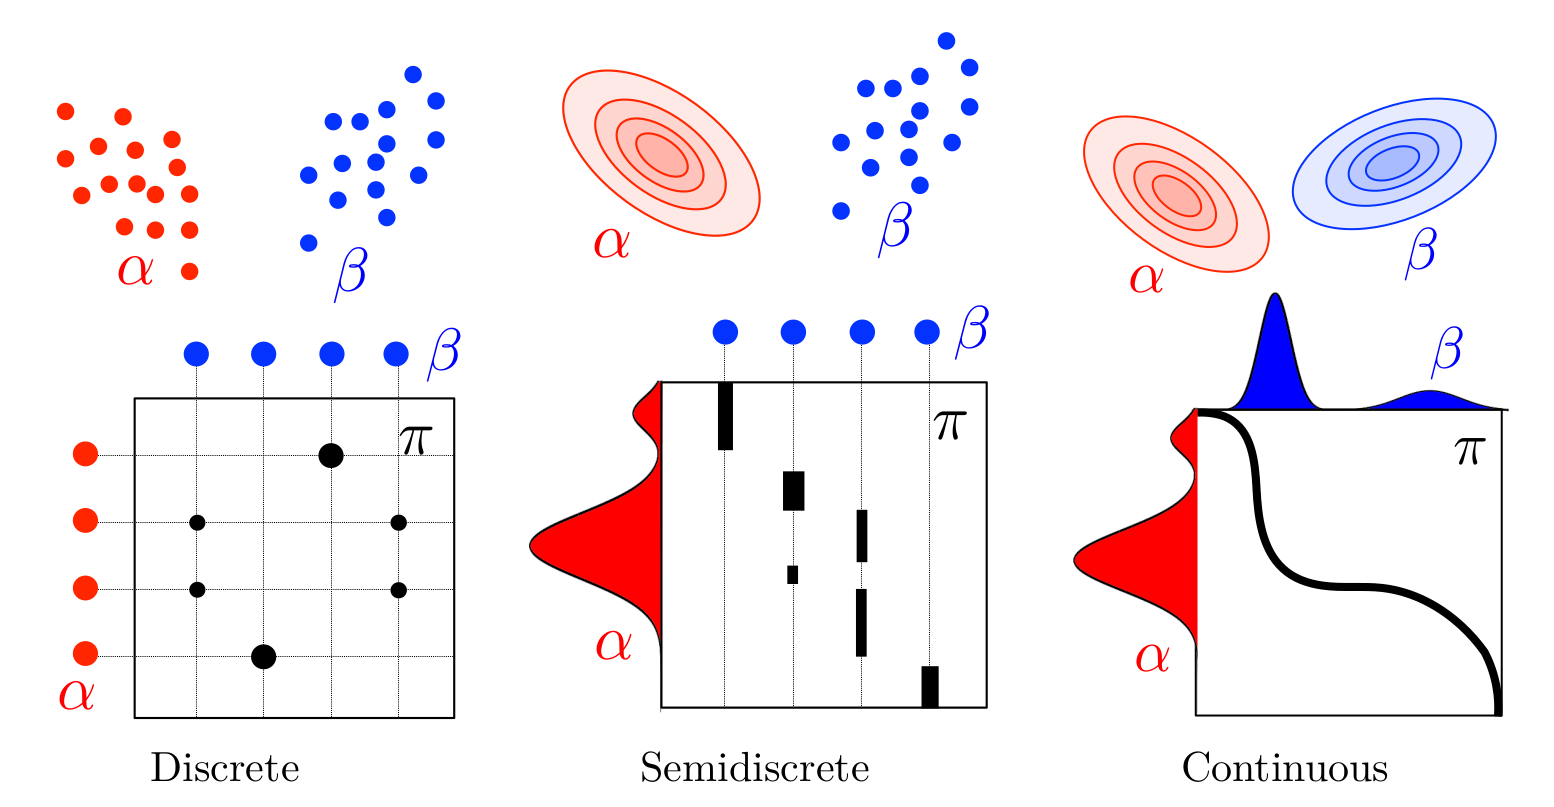
\includegraphics[width=\textwidth]{images/transport.png}
\end{frame}


\begin{frame}{Review: Optimal Transport}
  \begin{block}{General formulation}
    \[\mathcal L_C(\alpha, \beta) = \min_{\pi \in \mathcal U(\alpha,
        \beta)}\int_{\mathcal X\times \mathcal Y} c(x,y)d\pi(x,y)\]
  \end{block}
  \begin{block}{Probabilistic interpretation}
    \[\mathcal L_C(\alpha, \beta) = \min_{X, Y} \set{\mbm E(c(X,Y)) : X \sim \alpha,
        Y\sim \beta}\]
  \end{block}
  \begin{block}{Intuition}
    Optimal transport gives a distance measure between probability distributions.
  \end{block}
\end{frame}

\begin{frame}{Wasserstein Distance}
  A special case of optimal transport. ``A natural way to lift ground distance
  to distribution distance.''
  \begin{block}{Definition}
    Let $P_p(\Omega)$ be the set of Borel probability measures with finite $p$th
    moment defined on a given metric space $(\Omega, d)$. The $p$-Wasserstein
    metric $W_p$, for $p\geq1$, on $P_p(\Omega)$ between distribution $\mu$ and
    $\nu$, is defined as
    \[W_p(\mu, \nu)=\Big(\min_{\gamma\in \mathcal U(\mu, \nu)}\int_{\Omega\times
        \Omega}d^p(x,y)d\gamma(x,y)\Big)^{\frac{1}{p}}\]
  \end{block}
\end{frame}


\begin{frame}{1-Wasserstein Distance}
  \begin{block}{Primal Problem}
    \[KP(\mu, \nu)=\min_{\gamma}\int_{\Omega\times \Omega}d(x,y)d\gamma(x,y)\]
    \[s.t. \quad \int_Y d\gamma(x,y)=p(x), \int_X d\gamma(x,y)=q(y)\]
    \[\gamma(x,y)\geq 0\]
  \end{block}

  \begin{block}{Kantorovich-Rubinstein theorem}
    \[DP(\mu, \nu)=\max_{\phi\in Lip_1(X)}\int_X\phi(x)p(x)dx-\int_X\phi(x)q(x)dx\]
    \[DP(\mu, \nu)=\max_{\phi\in Lip_1(X)}\mb E_p\phi(x)-\mb E_q\phi(x)\]
    \[Lip_1(X)=\set{\phi : |\phi(x)-\phi(y)|\leq d(x,y)}, \forall x,y\in X\]
  \end{block}
\end{frame}


\begin{frame}{Algorithm for Optimal Transport}
  \begin{block}{Discrete problem: linear programming}
    Can be formulated as a minimum cost maximum flow problem.
    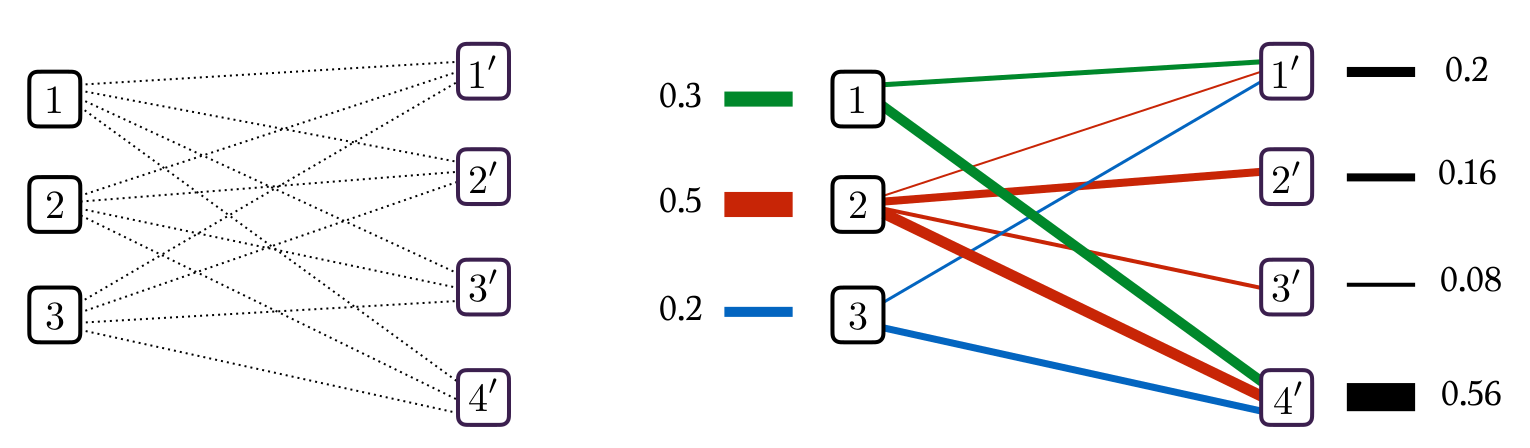
\includegraphics[width=\textwidth]{images/flow.png}
  \end{block}
\end{frame}

\begin{frame}{Any Questions?}
\end{frame}

\begin{frame}{Learning Wasserstein Embeddings}
  \begin{block}{Idea}
    \begin{itemize}
    \item Treat each data point as a distribution.
    \item Consider p-Wasserstein distance between data points.
    \item Embed Wasserstein space into Euclidean space.
    \item Learn this embedding with a neural network.
    \end{itemize}
  \end{block}
\end{frame}


\begin{frame}{Entropic Regularization} 
  \begin{block}{Kantorovish formulation}
    \[U(a, b) = \set{\b P\in \mb R_+^{n\times m} : \b P \mbm 1_m = \b a, \b P^T
        \mbm 1_n = \b b} \]
    $\b P_{i,j}$ denotes how much mass from $i$th point in $\b a$ is transported
    to the $j$th point in $\b b$. $U(a, b)$ is all valid transport plans. $\b P$
    is known as a coupling matrix.
  \end{block}

  \begin{block}{Entropy}
    Discrete entropy of a coupling matrix $\b P$:
    \[\b H(\b P) := -\sum_{i, j} \b P_{i,j}(\log(\b P_{i, j})-1)\]
    $\b H(\b P) = -\infty$ if any entry of $\b P$ is negative or $0$.
  \end{block}
\end{frame}


\begin{frame}{Entropic Regularization} 
  \begin{block}{property}
     $\b H$ is 1-strongly concave:
      \[\forall x,y, (\grad f(x) - \grad f(y))^T (x-y) \leq ||x-y||_2^2\]
      \[\forall x, -Hf(x) - I \mbox{ is positive semidefinite}\]
  \end{block}
  \begin{block}{idea}
    Larger $\b H(\b P)$ $\rightarrow$ distribution more uniform.

    We can use $\b H$ to regularize optimal transport.
    
    \[L_{\b c}(\b a,\b b) = \min_{\b P\in U(\b a, \b b)}\langle {\b P, \b C} \rangle\]
    \[L_{\b c}^\epsilon(\b a,\b b) = \min_{\b P\in U(\b a, \b b)}\langle {\b P,
        \b C} \rangle - \epsilon\b H(\b P)\]
  \end{block}
\end{frame}

\begin{frame}{Entropic Regularization} 
  \[L_{\b c}^\epsilon(\b a,\b b) = \min_{\b P\in U(\b a, \b b)}\langle {\b P,
      \b C} \rangle - \epsilon\b H(\b P)\]
  $L_{\b c}^\epsilon(\b a,\b b)$ is known as the \textbf{Sinkhorn divergence}.
  \begin{block}{Properties}
    \begin{enumerate}
    \item There exists unique solution $\b P_\epsilon$.
      \item When $\epsilon\to 0$, $\b P_\epsilon\to \b P$.
      \item When $\epsilon\to \infty$, $\b P_\epsilon\to \b a\b b^T$ (uniform distribution).
    \end{enumerate}
    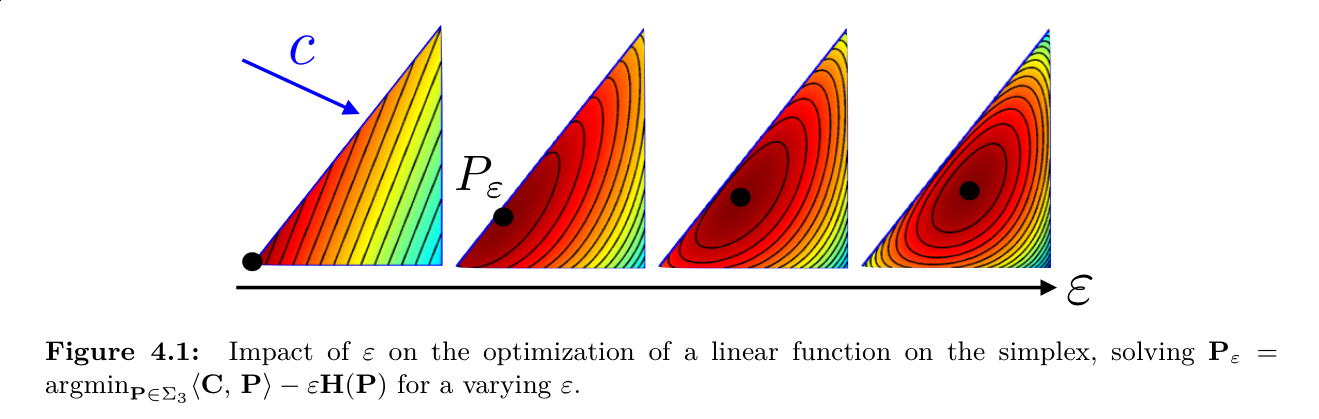
\includegraphics[width=\textwidth]{./images/entropy.png}
  \end{block}
\end{frame}

\begin{frame}{Entropic Regularization} 
  \begin{block}{Proposition (4.3)}
    Solution to the discrete entropic optimal transport problem
    \[L_{\b c}^\epsilon(\b a,\b b) = \min_{\b P\in U(\b a, \b b)}\langle {\b P,
        \b C} \rangle - \epsilon\b H(\b P)\]
    is unique and has the form
    \[\forall (i, j)\in [n]\times [m], \b P_{i, j}=\b u_i \b K_{i,j}\b v_j\]
    or equivalently,
    \[\b P = \mbox{diag}(\b u)\b K \mbox{diag}(\b v)\]
    where
    \[\b K_{i,j} = e^{-\b C_{i,j}/\epsilon}, (\b u,\b v)\in \mb R_+^n\times \mb R_+^m\]
    
  \end{block}
\end{frame}

\begin{frame}{Entropic Regularization} 
  \begin{block}{Sinkhorn iterations}
    \[\b P = \mbox{diag}(\b u)\b K \mbox{diag}(\b v)\]
    Adding constraints $\b P \mbm 1_m = \b a, \b P^T \mbm 1_n = \b b$,
    \[\b u \odot (\b K \b v) = \b a, \b v \odot (\b K^T \b u) = \b b\]
    This problem is known as ``matrix scaling'' and can be solved iteratively:

    \[\b u^{(l+1)} = \frac{\b a}{\b K \b v^{(l)}}, \b v^{(l+1)} = \frac{\b b}{\b K^T \b u^{(l+1)}} \]
    Note: this algorithm converges but possibly to different values for
    different initialization, since $(\lambda \b u, \b v/\lambda)$ is also a solution.
  \end{block}
\end{frame}

\begin{frame}{Entropic Regularization} 
  \begin{block}{Complexity}
    Let $n=m$ for simplicity, to achieve approximate transport plan $\hat{\b P}\in U(\b a, \b b)$ with
    $\langle {\hat{\b P}, \b C} \rangle \leq L_{\b C}(\b a, \b b) + \tau$, the
    time complexity is
    \[O(n^2\log n \tau^{-3})\]
  \end{block}

  \begin{block}{Remarks}
    The Sinkhorn iteration approximates optimal transport. Given enough time, it
    can give arbitrarily close approximations.
  \end{block}
\end{frame}

\begin{frame}{Any Questions?}
\end{frame}

\begin{frame}{Learning Entropic Wasserstein Embeddings}
  \begin{block}{Idea}
    \begin{itemize}
      \item Want ``similar'' data points to be close in a embedding space.
      \item Use a Wasserstein space as the embedding space.
      \item Use Sinkhorn iteration as a layer in the neural network.
    \end{itemize}
  \end{block}
\end{frame}

\end{document}
